Per quanto riguarda le pagine interne di un sito web, gli assi informativi obbligatori riassunti nelle "6 w" cambiano.\\
Infatti restano obbligatori gli assi Where, Who e What, mentre diventano opzionali gli assi Why, When e How. Analizziamo in generale come le pagine interne rispondono agli assi informativi:
	\begin{itemize}
		\item \textbf{Where}: a mio avviso l'utente è difficilmente in grado di capire dove si trova, sia per l'utilizzo incongruente del breadcrumb, sia per la struttura eterogenea delle pagine interne. Questo disorientamento si accentua soprattutto per le voci dei menù che reindirizzano a pagine web di altri siti (per esempio quelli che reindirizzano al portale principale dell'ateneo Aldo Moro)\begin{center}
\begin{figure}[h!]
           \begin{center}
           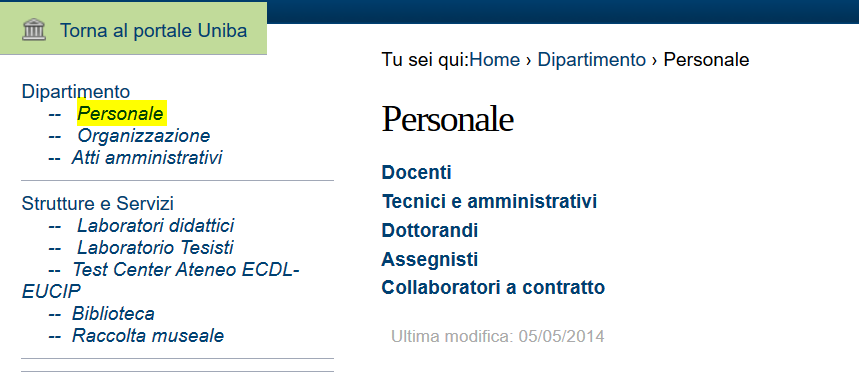
\includegraphics[scale=0.40]{C:/Users/elepo/Desktop/UNI/WIM/ANALISI_SITO/Relazione/sez/Pag_interne/b1.png}
           \caption{Breadcrumb di tipo 1}
           \end{center}
  \end{figure}
\end{center}

\begin{center}
\begin{figure}[h!]
           \begin{center}
           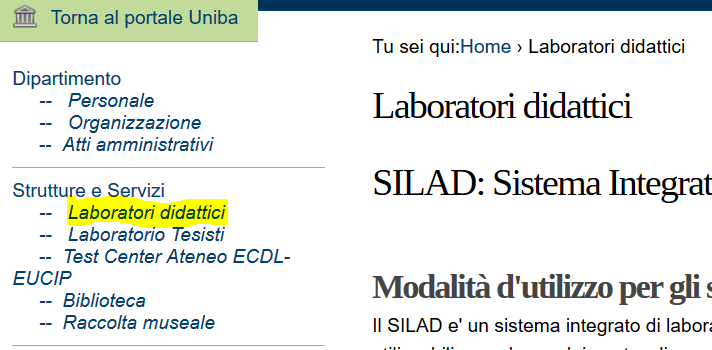
\includegraphics[scale=0.40]{C:/Users/elepo/Desktop/UNI/WIM/ANALISI_SITO/Relazione/sez/Pag_interne/b2.png}
           \caption{Breadcrumb di tipo 2}
           \end{center}
  \end{figure}
\end{center}
		\item \textbf{Who}: il logo continua a essere presente nell'header, pertanto anche a questa domanda l'utente trova una risposta;
		\item \textbf{What}: anche in questo caso il contenuto è abbastanza dichiarativo da poter rispondere alla domanda.
	\end{itemize}

Per quanto riguarda invece gli assi opzionali:
	\begin{itemize}
		\item \textbf{Why}: essendo un portale web dedicato a una struttura universitaria la pagina non ha "concorrenza" da parte degli altri siti, pertanto la pagina non è interessata a fornire alcun tipo di informazione in merito ai benefici nel suo utilizzo;
		\item \textbf{When}: La data degli ultimi aggiornamenti delle pagine interne è sempre presente e risponde all'asse informativo. Purtroppo però le date riportate per gli aggiornamenti sono molto antecedenti: questo è un fattore negativo riscontrato anche nella homepage che da un senso di staticità al sito.
		\item \textbf{How}: il come arrivare alle sottosezioni delle pagine interne o in generale come reperire una certa informazione non è per nulla chiaro a causa della eterogeneità della struttura delle pagine.
	\end{itemize}